\section{Experiment}

\paragraph{Basic setup}

We perform all our measurements using a torsion axis (Fig. \ref{fig::torsion}).
Analogous to the feather constant, a spiral spring has a specific torsion coefficient $D$.
As we do not know $D$, we have to find its value before performing further experiments.

\begin{figure} [ht]
	\centering
	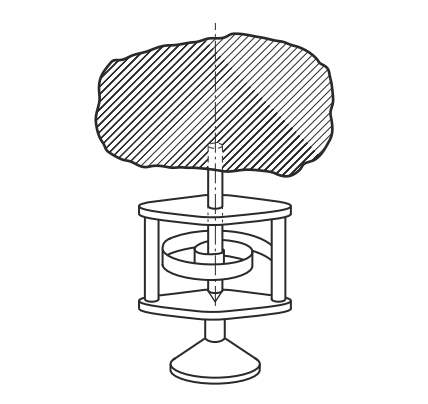
\includegraphics[width=120pt]{img/torsion_axis.PNG}
	\caption{Torsion axis \cite{manual}}
	\label{fig::torsion}
\end{figure}

In order to do that, we place two identical, quadratic beams of known length $b$, width $c$ and weight $M$ on the torsion axis perpendicular to the principle axis of the two beams (as in Fig. \ref{fig::steiner} with $d = 0$).
We now measure the oscillation period $T_1$ of this system.
To increase accuracy we measure multiple periods and divide by the number of periods and do this multiple times.
Period measurements are performed that way for the whole experiment.
Next we add a circular disk, again of known radius $R_S$ and weight $M_S$, on top of the two beams and measure the oscillation period $T_2$ of this new system.
From those measurements we are able to calculate $D$.

\begin{figure} [ht]
	\centering
	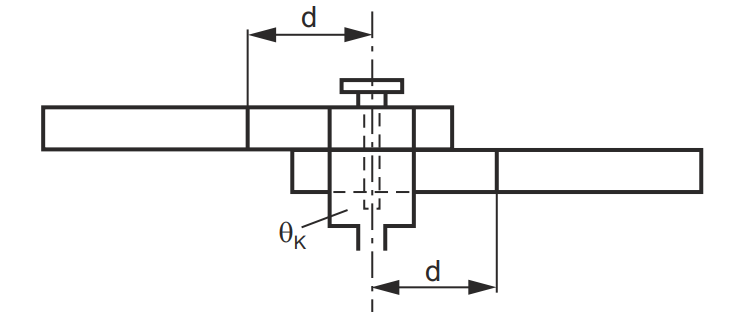
\includegraphics[height=120pt]{img/steiner.PNG}
	\caption{Setup to verify Steiner's theorem \cite{manual}}
	\label{fig::steiner}
\end{figure}

\paragraph{Verifying Steiner's theorem}
In order to verify Steiner's theorem we use the same two beams as before.
This time, we move the two bars step by step in opposite directions as shown in Fig. \ref{fig::steiner} and measure the oscillation periods $T_a$ of the system.
We increase the distance $d$ by $5$cm for every measurement, going from $0$cm to $25$cm.

\paragraph{Ellipse of inertia}

In order to show that the moment of inertia forms an ellipse if rotated in a plane place a weight with a scale ring (Fig. \ref{fig::ring}) on to our torsion axis.
For every measurement $T_S$ of the oscillation period we increase the angle of the weight by $10$\textdegree, between $0$\textdegree \space and $90$\textdegree.

\begin{figure} [ht]
	\centering
	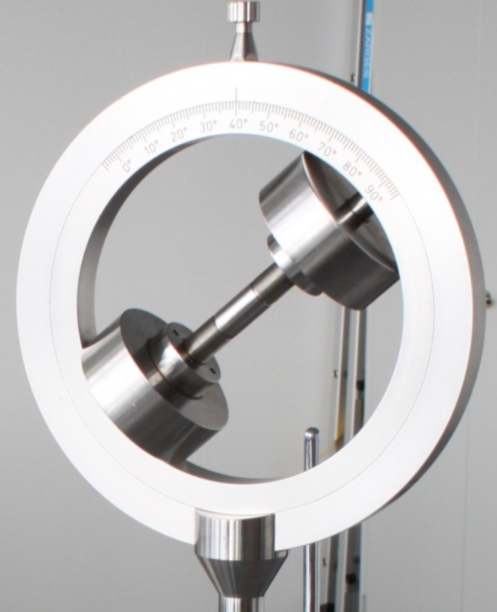
\includegraphics[height=120pt]{img/scale_ring.PNG}
	\caption{Weight in scale ring \cite{website}}
	\label{fig::ring}
\end{figure}
